\section{Introduction}

Spherical systems are still a niche format in robotics for the use of mobile mapping, compared to more prominent systems like unmanned aerial vehicles (UAV) or rovers.
The majority of research in that area focuses on the locomotion mechanism to move the ball around~\cite{Chen2013, Ylikorpi2007, Chase2012, Joshi2010, Anwar2014}.
Often, these approaches use actuators inside the ball, e.g., moving masses or conservation of angular momentum via flywheels, and study the mobility, controllability, and corresponding path planning methods.
Others focus more on the mathematical description of the motion of the ball itself~\cite{Hogan2015Modeling, Mamaev2020Dynamics, Burkhardt2016Reduced, omark2020, fiori2024lie}. 
However, there is a lack of research that focuses on the use of spherical systems for mobile mapping using its internal sensors.
Some authors~\cite{s22041413, Li2023Special, Bruhn2008A}, including the European Space Agency~(ESA)~\cite{ESA}, have suggested the suitability of the ball-shaped design for exoplanetary explortion and exploration of other inaccessable, dangerous, or harsh terrestrial environments like mine shafts or narrow funnels.
The advantages of spherical systems in that context include protection of the internal sensors, an advantage in maneuverability and mass efficiency, and a locomotion principle that leads to sensor coverage without needing additional actuators for the sensor.
However, one major disadvantage considering mobile mapping are the large angular velocities and agressive system dynamics, which introduce degrading effects on inertial measurement units (IMUs), LiDAR sensors, and cameras.
In our previous work, we have built spherical mobile mapping prototypes including LiDAR sensors and IMUs, assuming that each sensor would be mounted in the balls center~\cite{9591183, ARZBERGER2021100004, 10256359}.
\begin{figure}
  \centering
  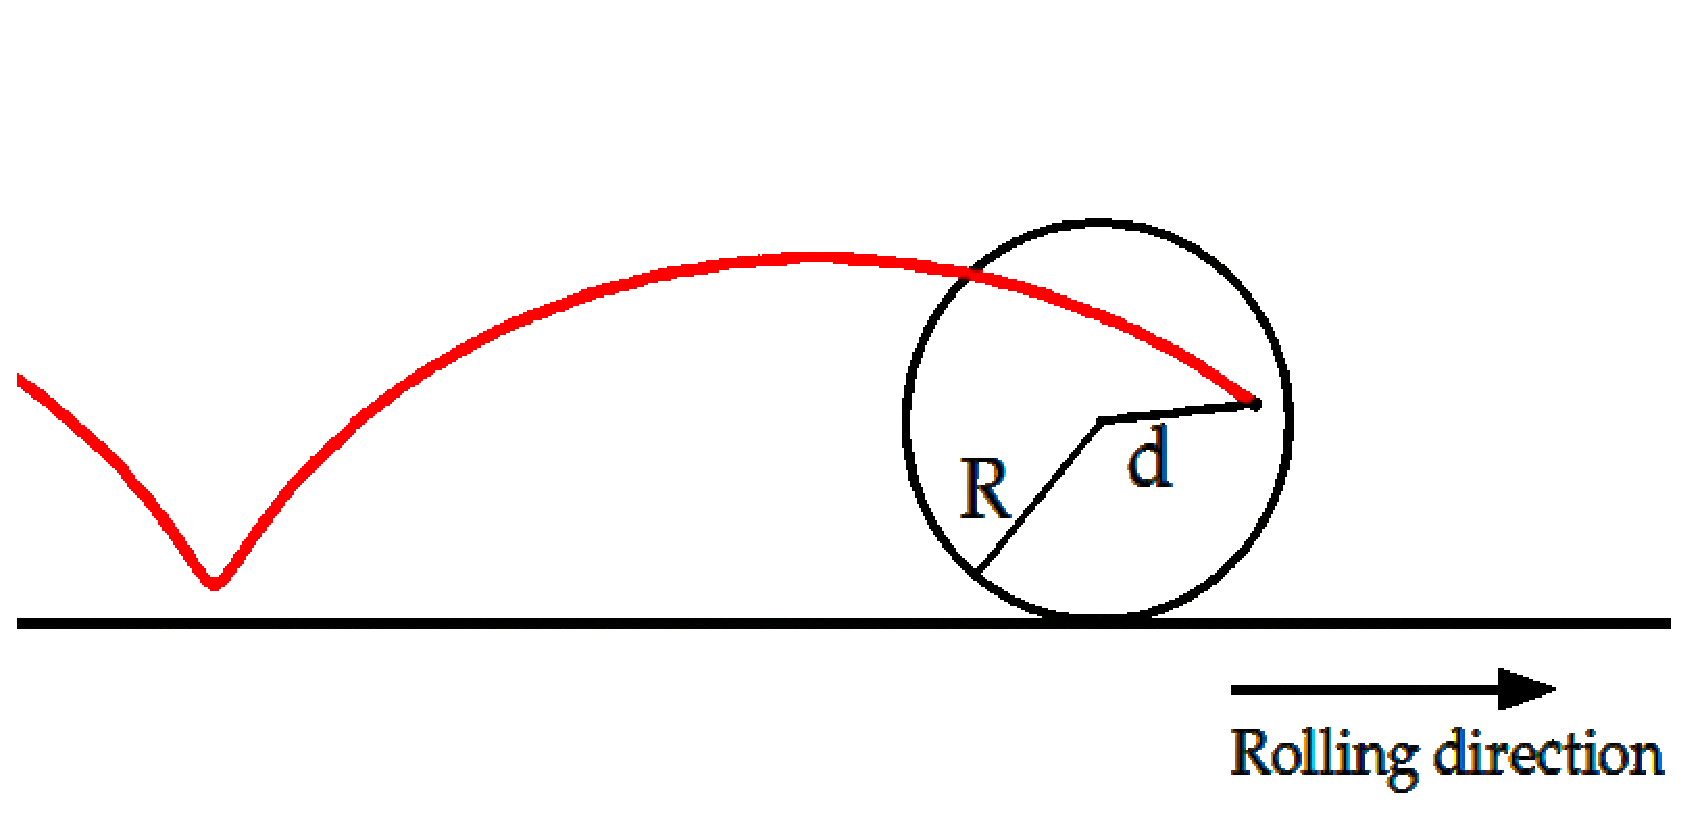
\includegraphics[width=\linewidth]{img/trochoidanim}
  \caption{Trochoid anim.}
  \label{fig:trochoidanim}
\end{figure}
In reality, though, the trajectory of a sensor mounted rigidly inside the ball resembles a curate trochoid, which is illustrated in Figure~\ref{fig:trochoidanim}.
We approach this problem in our paper, having the following contributions:
\begin{itemize}
  \item A motion model that estimates the trochoidal 6-DoF trajectory of a sensor mounted rigidly inside the spherical system, based on IMU measurements and an extrinsic calibration of the sensor with respect to the balls center.
  \item A calibration procedure for LiDAR sensors that estimates the extrinsic translation parameters of the sensor with respect to the balls center.
  \item A comparison of the motion model with two state-of-the-art Lidar-Inertial odometry (LIO) methods, illustrating their difficulty to produce trochoidal trajectories.
\end{itemize}
The rest of the paper is structured as follows: 
In the next section, we introduce other work related to extrinsic LiDAR calibration and LiDAR-inertial odometry.
Then, we introduce our own calibration procedure for spherical mobile mapping systems, followed by the introduction of our 3D trochoidal motion model.
Afterwards we perform experiments with our spherical prototype and discuss the quality of the resulting trochoidal trajectories, followed by conclusions and possible future work.

 